\section{Resultados}

Los hallazgos obtenidos evidencian lo siguiente: Estos resultados refuerzan la importancia de integrar metodologías y arquitecturas sólidas en el desarrollo moderno de software.

\subsection{Programación Orientada a Objetos (POO) y Modelo–Vista–Controlador (MVC)}
Ambos enfoques aportan modularidad y escalabilidad al desarrollo de software, ya que favorecen la separación de responsabilidades y la organización del código \cite{poo}\cite{mvc}. En este proyecto se utilizó Java como lenguaje principal, aprovechando sus características orientadas a objetos para estructurar de manera clara y adaptable los componentes del sistema.

\subsection{Frameworks backend (Node.js y Spring Boot)}
Node.js destaca por su eficiencia en aplicaciones de microservicios y entornos que requieren alta escalabilidad, mientras que Spring Boot ofrece mayor solidez y seguridad en proyectos empresariales \cite{nodejs_springboot}. En el caso del presente trabajo, se optó por emplear Spring Boot debido a su facilidad de configuración y a las ventajas que proporciona en entornos corporativos. Aunque no se implementó bajo un modelo de microservicios, se desarrolló una arquitectura monolítica bien estructurada que permitió cumplir con los objetivos formativos del sistema.

\begin{figure}[h]
\centering
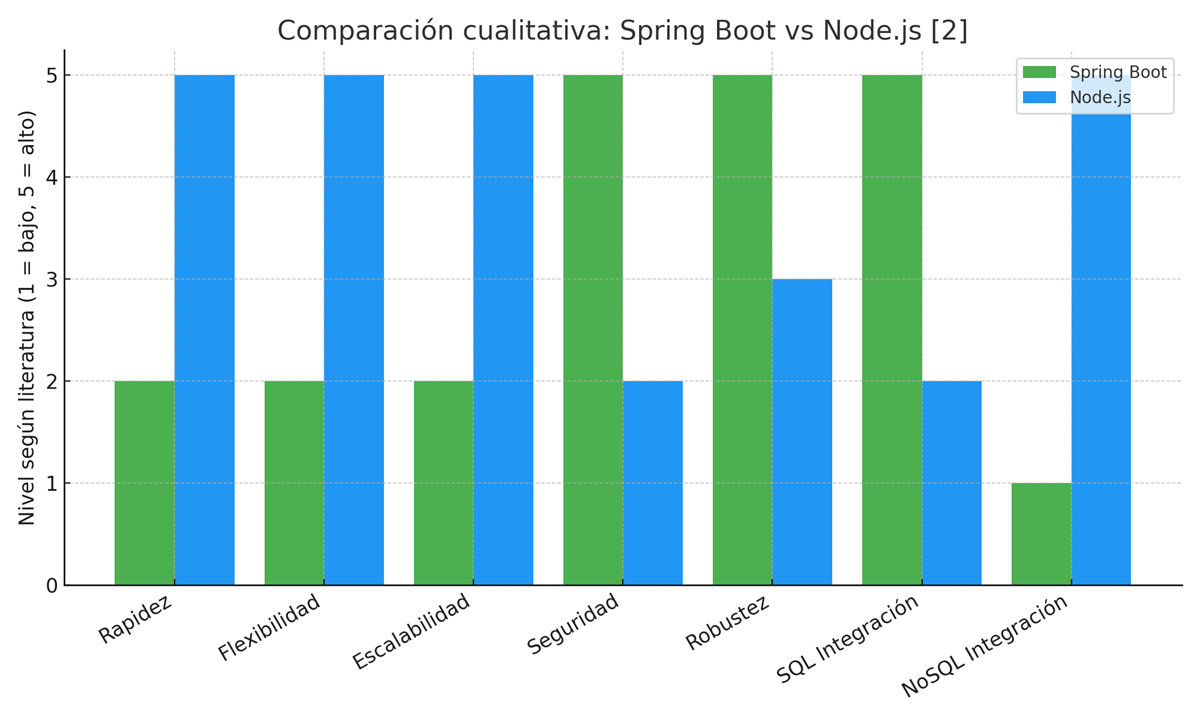
\includegraphics[width=0.3\textwidth]{graphics/node.js vs spring boot.png}
\caption{Comparación entre Node.js y Spring Boot en el desarrollo backend.}
\label{fig:nodejs_springboot}
\end{figure}

\subsection{Metodología Scrum}
Este marco de trabajo fortalece la comunicación y la colaboración en equipo, además de facilitar la entrega incremental de valor \cite{scrum}. En el proyecto no se adoptó Scrum en su totalidad, pero se aplicaron prácticas inspiradas en esta metodología, como la organización de tareas mediante un modelo tipo Canva para estructurar los Sprints y dar seguimiento a los avances de manera iterativa.

\begin{figure}[h]
\centering
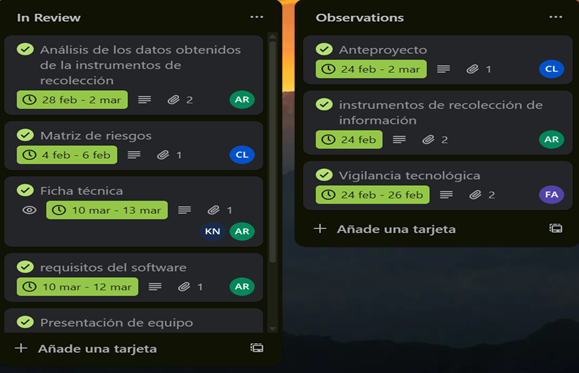
\includegraphics[width=0.3\textwidth]{graphics/Prueba de scrum.png}
\caption{Implementación de la metodología Scrum en el proyecto.}
\label{fig:scrum}
\end{figure}

Y de igual manera implementamos los dailys en llamadas en Discord.

\begin{figure}[h]
\centering
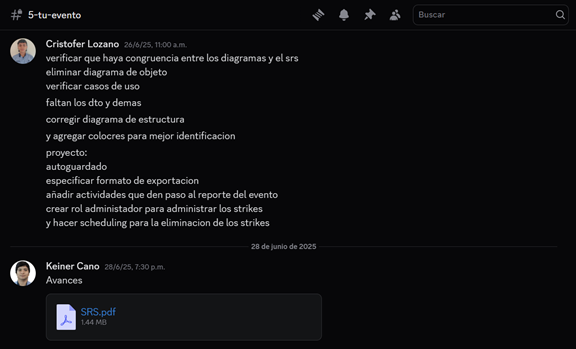
\includegraphics[width=0.3\textwidth]{graphics/discord.png}
\caption{Comunicación diaria en Discord para el seguimiento del proyecto.}
\label{fig:discord}
\end{figure}

\subsection{Las bases de datos}
Las bases de datos relacionales continúan siendo esenciales, aunque las NoSQL amplían el espectro en escenarios, para nuestro proyecto el uso de Fetch es útil para las comunicaciones y usamos NoSQL en los entornos móviles y web, para hacer comunicación entre la API y la base de datos haciendo cuerpos JSON desde el Frontend, para el proyecto de eventos usamos una base de datos con el motor SQL de PostgreSQL.

\begin{figure}[h]
\centering
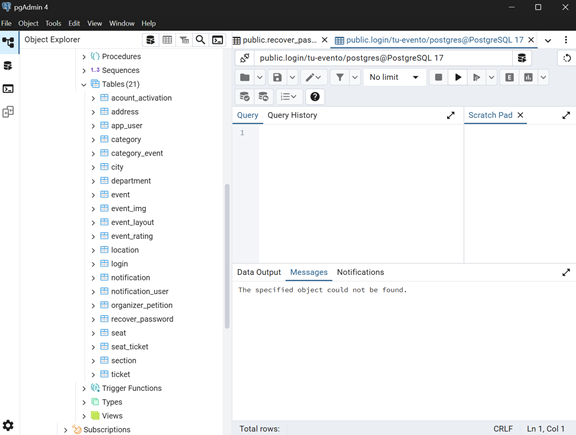
\includegraphics[width=0.3\textwidth]{graphics/base de datos postgres.png}
\caption{Estructura de la base de datos PostgreSQL utilizada en el proyecto.}
\label{fig:postgres}
\end{figure}

Estos resultados refuerzan la importancia de integrar metodologías y arquitecturas sólidas en el desarrollo moderno de software.